\clearpage
\subsection{Equal source and target counts: relaxed stopping and an
$\varepsilon\times N$ grid}
\label{sec:equal-count-grid}
This section uses $\kappa=0.8$ only. The source and target now have the
same number of points $N$; earlier runs fixed the target at $1600$ points.
Write $N=m_N^2$ and $\varepsilon=1/(8m_\varepsilon)$. The joint-movement
schedule $\varepsilon=1/(8\sqrt N)$ is then the diagonal $m_\varepsilon=m_N$
of the grid, and the fixed-$\varepsilon$ sweep is the row
$\varepsilon=1/320$ ($m_\varepsilon=40$). Both experiments are slices of
one grid with $m_N\in\{10,14,20,28,40,57,80\}$ ($N=100$ to $6400$) and
$m_\varepsilon$ from $5$ to $1280$ ($\varepsilon=1/40$ to $1/10240$),
spaced by roughly $\sqrt2$. Costs are evaluated at
$\varepsilon_{\mathrm{eval}}=1/320$ as before.

\paragraph{Relaxed stopping rule.}
The optical Sinkhorn solve previously stopped at marginal $L^1$ error
$10^{-7}$ and potential change $10^{-5}$. We now stop at marginal error
$10^{-3}$ and potential change $10^{-3}$. The evaluation EOT solves keep
tolerance $10^{-9}$. To decide whether this is safe, we compare the
refractor itself rather than the cost. The refractor
$R(x)=\exp\bigl(\operatorname{softmin}_j(g_j-c(x,y_j))\bigr)$ is defined up
to scale, so we report
\[
 \delta_R=\max_x\Bigl|\Delta\log R(x)-\textstyle\sum_x p(x)\,\Delta\log R(x)\Bigr|,
\]
the maximum relative change in radius after removing the scale, together
with the largest change in surface normal and in refracted ray direction.
The acceptance bar is $\delta_R\le 10^{-3}$ ($0.1\%$).
Table~\ref{tab:relaxed-stopping} compares the relaxed rule with the strict
rule. The change in the surface grows linearly with the marginal tolerance,
$\delta_R\approx0.08\times$ the marginal tolerance, and does not grow with
$N$. At the chosen setting $\delta_R\le8.1\times10^{-5}$, normals move at
most $0.036^\circ$ and rays at most $0.011^\circ$, a margin of about
$12\times$ below the bar, while each solve runs $1.5$--$3\times$ faster.
The potential-change tolerance was almost never the binding criterion.
The debiased divergence is more sensitive than the surface
(up to $2\%$ relative change at $\varepsilon=1/80$, $N=400$), because it is
a difference of nearly equal terms.

\begin{table}[h]
 \centering
 \begin{tabular}{rrrrrrr}
  $N$ & $\varepsilon$ & strict (min) & relaxed (min) & $\delta_R$ &
  normal ($^\circ$) & ray ($^\circ$)\\ \hline
  400 & 1/80 & 0.5 & 0.3 & $6.9\times10^{-5}$ & 0.031 & 0.008\\
  400 & 1/320 & 1.1 & 0.5 & $6.3\times10^{-5}$ & 0.026 & 0.007\\
  400 & 1/1280 & 3.9 & 1.3 & $8.0\times10^{-5}$ & 0.036 & 0.011\\
  1600 & 1/320 & 16.4 & 6.9 & $7.4\times10^{-5}$ & 0.031 & 0.008\\
  1600 & 1/1280 & 61.2 & 20.0 & $8.1\times10^{-5}$ & 0.035 & 0.010\\
  3600 & 1/480 & 121.6 & 49.8 & $8.0\times10^{-5}$ & 0.035 & 0.009\\
 \end{tabular}
 \caption{Strict stopping (marginal $10^{-7}$, change $10^{-5}$) against
 relaxed stopping (marginal $10^{-3}$, change $10^{-3}$), $\kappa=0.8$,
 source count = target count. Times are wall minutes per cell (hard and
 entropic solves plus debiased evaluation).}
 \label{tab:relaxed-stopping}
\end{table}

\paragraph{Grid coverage.}
We keep only cells predicted to take under three hours with the relaxed
rule. This leaves 106 of the 119 grid cells. The excluded cells are the large-$N$,
small-$\varepsilon$ corner; in particular $N=6400$ is run only at
$\varepsilon\ge1/456$, so the joint-movement diagonal stops at $N=3249$.
Figure~\ref{fig:equal-count-lines} shows the two experiments and
Figure~\ref{fig:equal-count-eps-lines} the whole grid, one line per $\varepsilon$.

\begin{figure}[p]
 \centering
 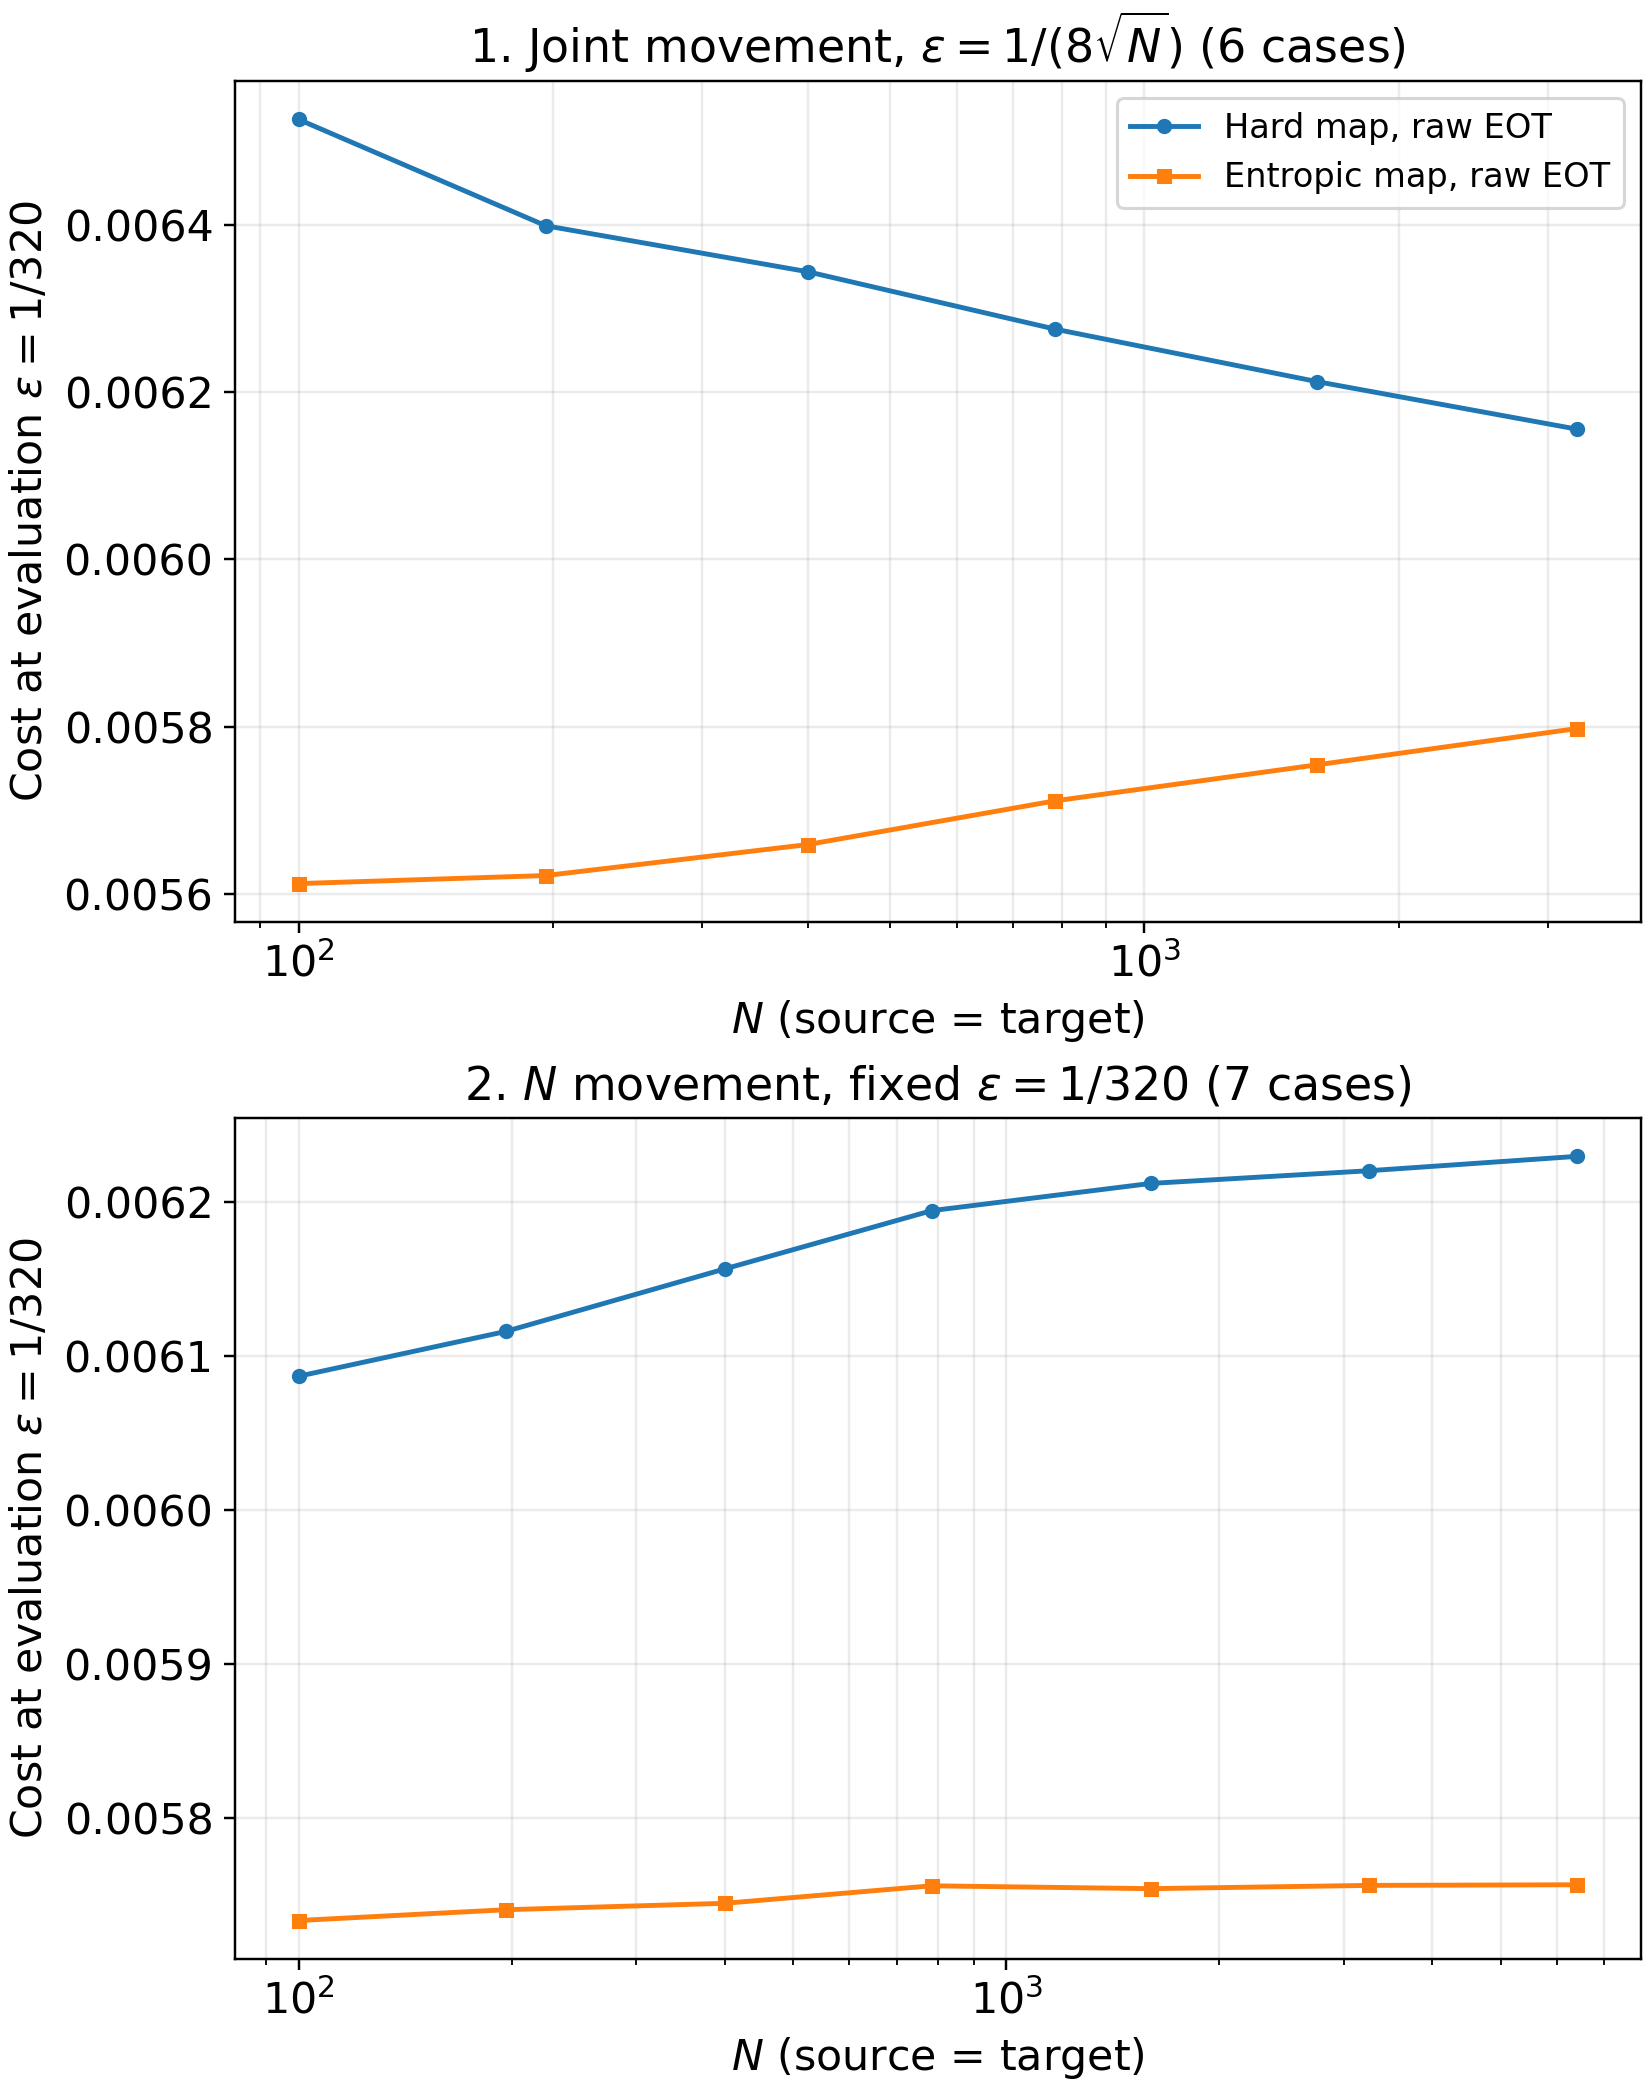
\includegraphics[width=.8\textwidth]{equal_count_joint_and_n.png}
 \caption{\large $\kappa=0.8$, source count = target count, relaxed
 stopping. Top: joint movement $\varepsilon=1/(8\sqrt N)$. Bottom: $N$
 movement at fixed $\varepsilon=1/320$. Raw EOT cost for the hard and
 entropic maps, evaluated at $\varepsilon=1/320$.}
 \label{fig:equal-count-lines}
\end{figure}

\begin{figure}[p]
 \centering
 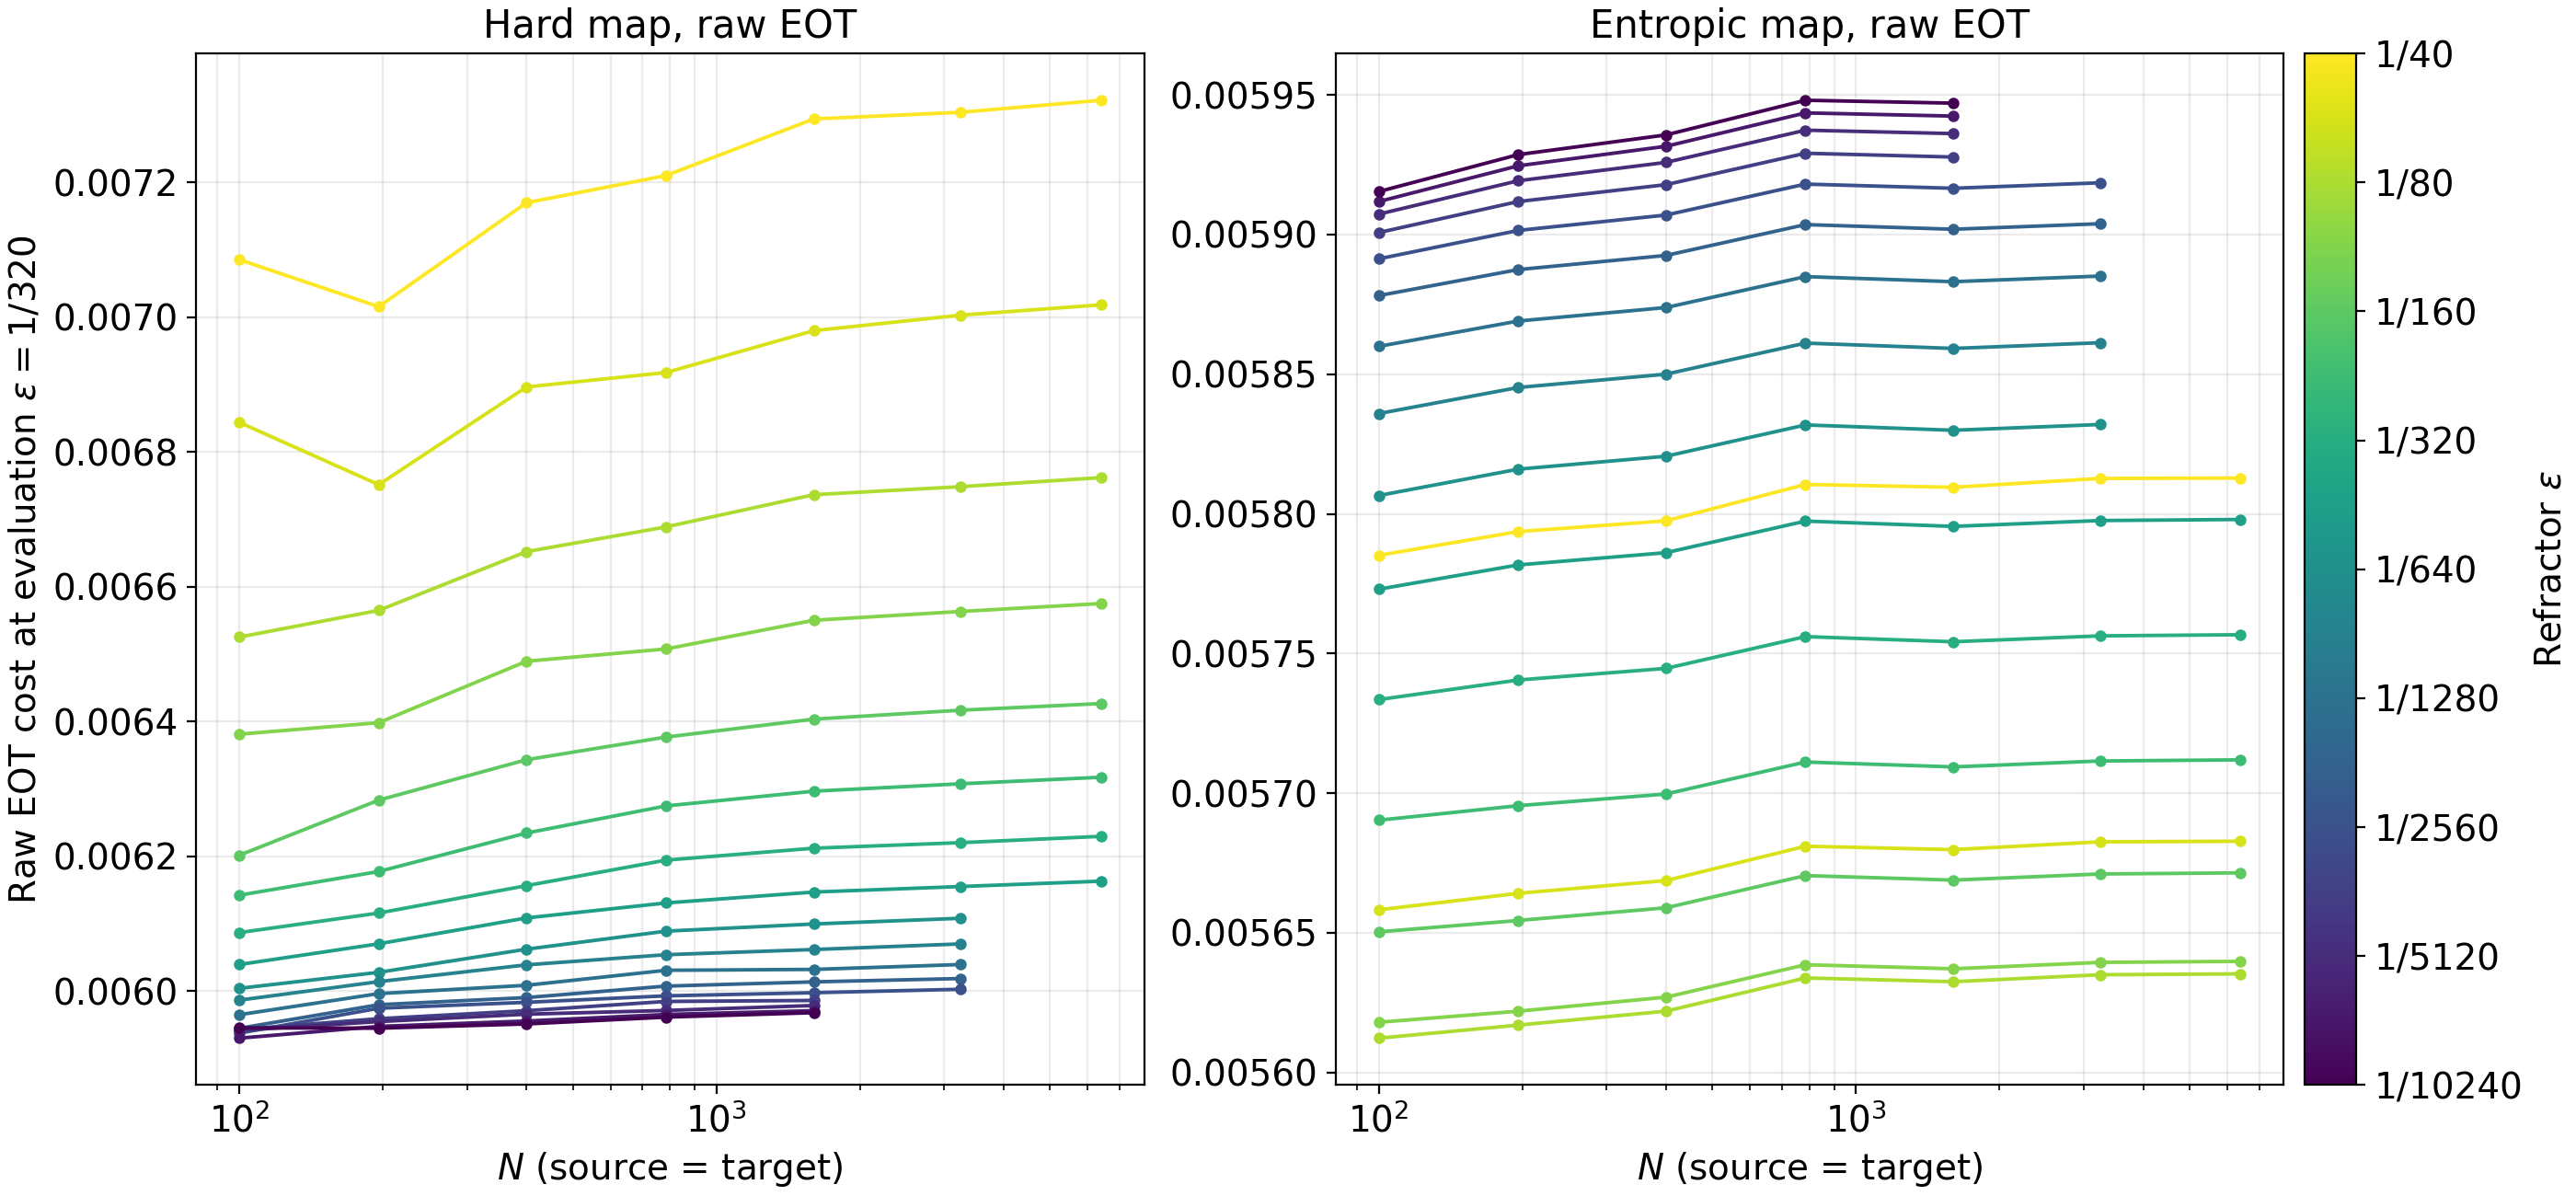
\includegraphics[width=\textwidth]{equal_count_eps_lines.png}
 \caption{\large $\kappa=0.8$, source count = target count: raw EOT
 cost (evaluated at $\varepsilon=1/320$) against $N$, one
 line per refractor $\varepsilon$. Left: hard map. Right: entropic map.
 Lines stop where larger $N$ was predicted to take over three hours.}
 \label{fig:equal-count-eps-lines}
\end{figure}
